\documentclass{beamer}
\usepackage[utf8]{inputenc}
\usepackage[russian]{babel}
\usepackage{graphicx}
\usepackage{epsf,amsmath,amsfonts,amssymb,amsbsy}
\usepackage[mathscr]{eucal}
\usepackage{pgfplots}
\pgfplotsset{width=10cm,compat=1.9}
\textheight=255mm
\def\andname{\hspace*{-2.3mm},}
\def\baselinestretch{0.9}
\newcommand*\rfrac[2]{{}^{#1}\!/_{#2}}
\usefonttheme{structuresmallcapsserif}
\usetheme{Copenhagen}
\graphicspath{{pictures/}}
\DeclareGraphicsExtensions{.pdf,.png,.jpg}
\title[Radio Pulsars]{\small Introduction to Radio Pulsars}
\author{Nikita Prokopenko}
\institute{MIPT}
\date[MIPT 2021] % (optional)
{February 2022}

\begin{document}

\frame{\titlepage}
\begin{frame}
\frametitle{Presentation Plan}

\begin{itemize}
\item A brief history of the discovery
\end{itemize}
\begin{itemize}
\item Vacuum model
\end{itemize}
\begin{itemize}
\item The zeroth-order model
\end{itemize}

\end{frame}

\begin{frame}
\frametitle{A brief history}
\begin{columns}
 
\column{0.6\textwidth}
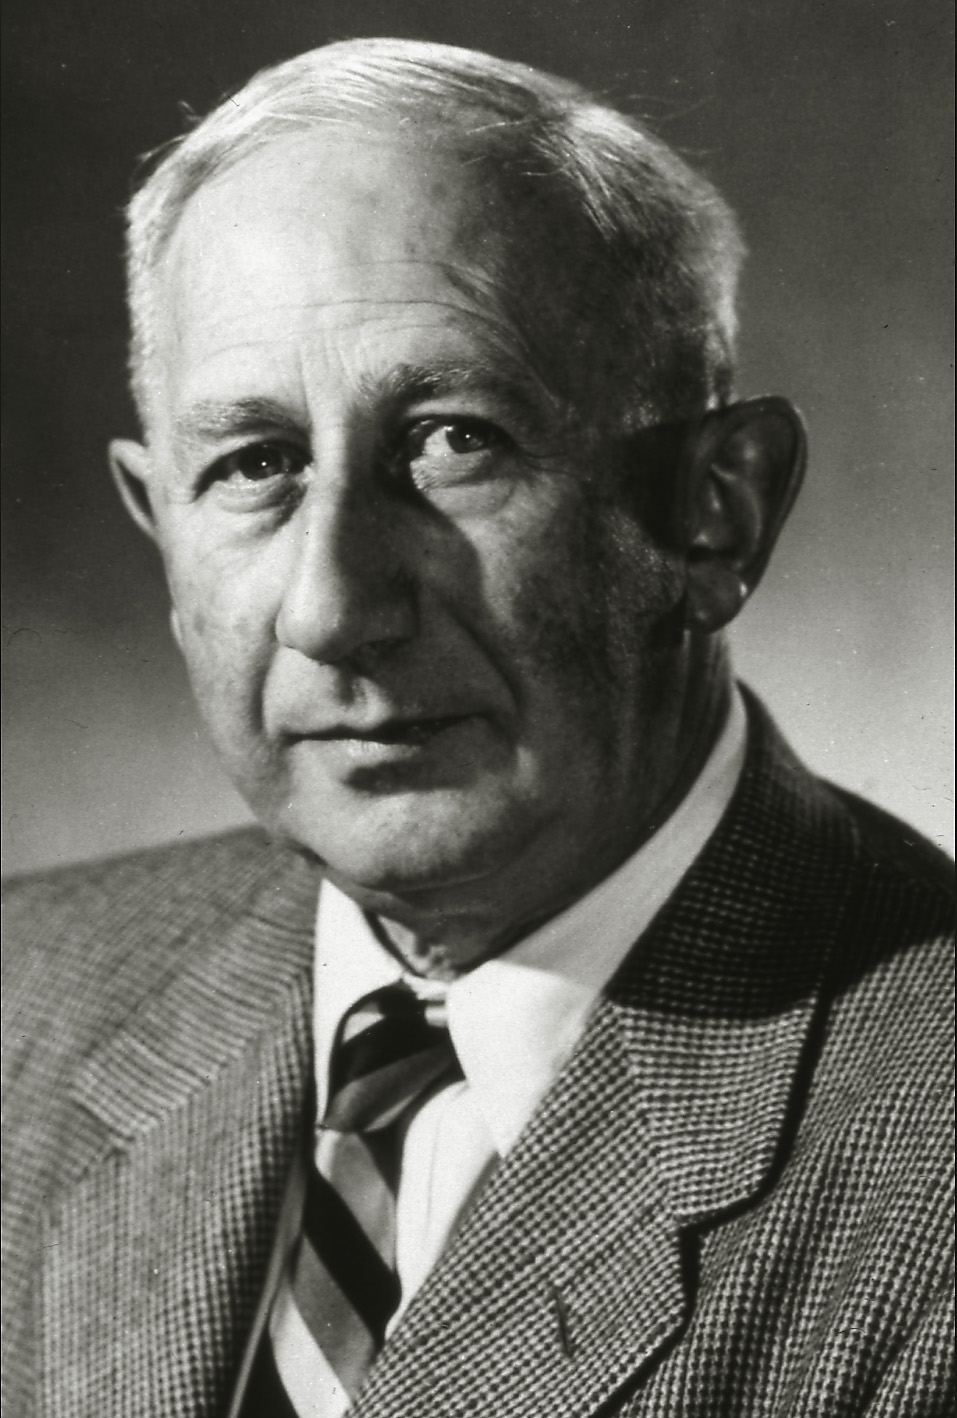
\includegraphics[width=.32\textwidth,height=2.8cm]{Walter-Baade_Astronom.jpg}\hfill%
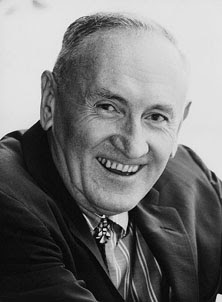
\includegraphics[width=.32\textwidth,height=2.8cm]{Zwicky.jpg}\hfill%
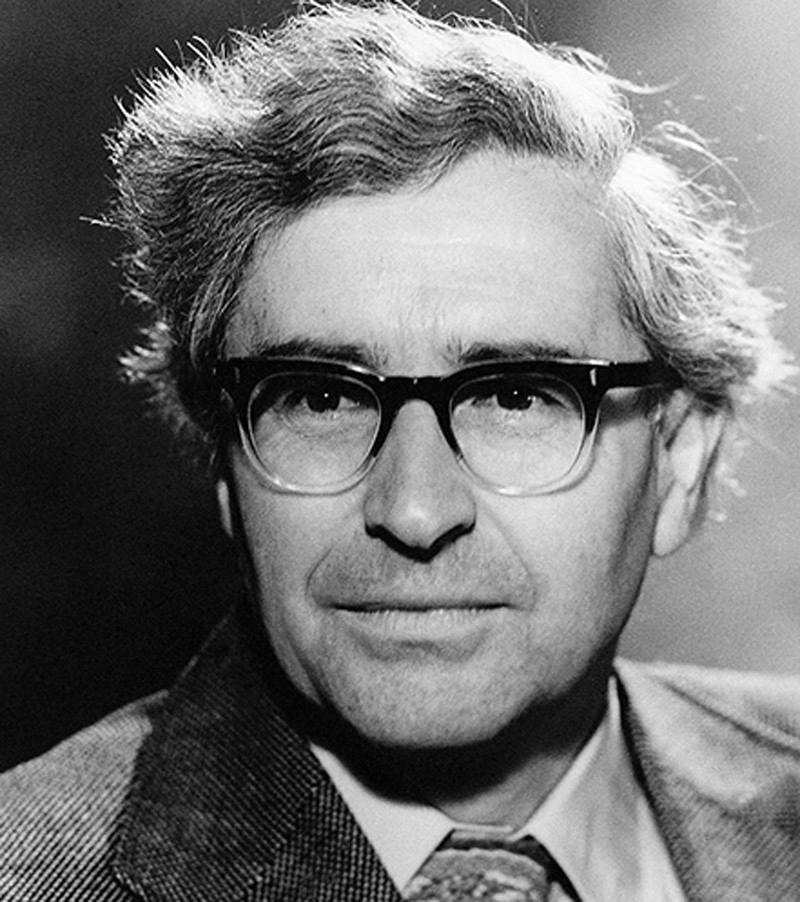
\includegraphics[width=.32\textwidth,height=2.8cm]{d41586-021-02617-0_19678262.jpg}\\

\column{0.5\textwidth}
\begin{itemize}
\item Prediction - [Baade, Zwicky, 1934; Landau 1932]
\end{itemize}
\begin{itemize}
\item Discovery - [Hewish et al., 1968]   \end{itemize}
Basic parameters:
\begin{itemize}
\item $M \approx 2 \cdot 10^{33} \text{g}$ 
\item $R = 10 \div 15 km$
\item $P = 1.5 ms$
\item $B_0 \sim 10^{12} Gs$
\end{itemize}

 
\end{columns}

\end{frame}
\begin{frame}
\frametitle{Vacuum model}
\begin{columns}
\column{0.4\textwidth}
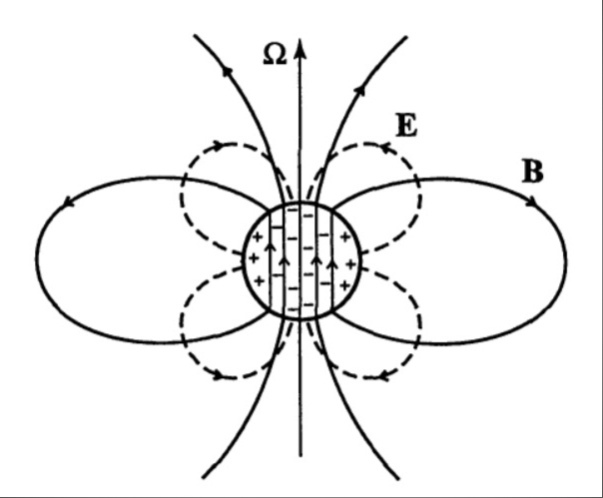
\includegraphics[scale=0.22]{UWkNMChBQPQ.jpg}


\column{0.64\textwidth}
Inside a well-conducting sphere:
$$\textbf{E}_{in} + \frac{\bf{\Omega} \times \bf{r}}{c} \times \textbf{B}_{in} = 0$$
Let the axis of rotation is parallel to the axis of magnetization, so:
\\ 


$\Phi_e(r < R, \theta) = \frac{1}{2}\frac{\Omega\text{B_0}}{c}r^2 \sin^2{\theta}$

$\Phi_e (r > R, \theta) = -\frac{1}{3}\frac{\Omega B_0}{c} \frac{R^5}{r^3} P_2( \cos{\theta})$
\end{columns}
\end{frame}



\begin{frame}
\frametitle{The zeroth-order model}
Сurvature of the force lines of the dipole magnetic field $\implies$ radiation of hard gamma quanta
\\

$\gamma + B \rightarrow e^{+} + e^{-} + B$ [Sturrock, 1971]
\\

A chain of processes:
\begin{itemize}
    \item acceleration of primary particles
    \item radiation of bending photons
    \itemthe birth of secondary electron-positron pairs
    \item acceleration of secondary particles, radiation of bending photons by them
    \item screening of the longitudinal electric field
\end{itemize}


\end{frame}

\begin{frame}
\begin{columns}

\column{0.64\textwidth}
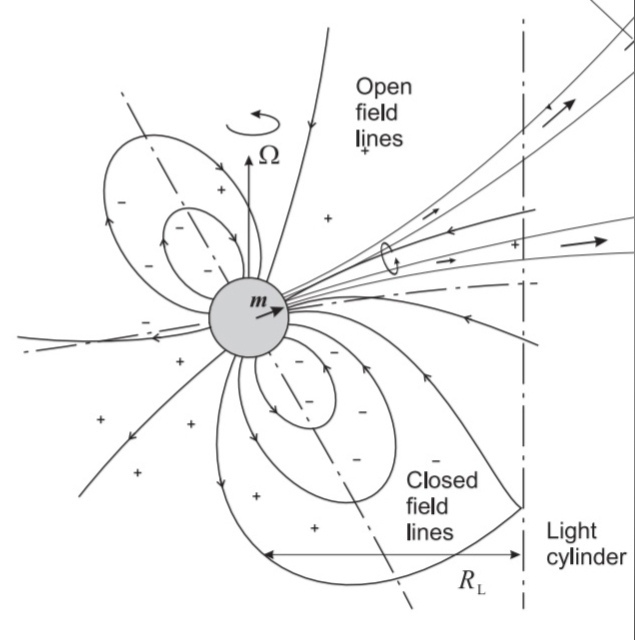
\includegraphics[scale=0.3]{fVHrmo5Z7Z0.jpg}
\column{0.64\textwidth}
\frametitle{Structure of the magnetosphere}
A magnetosphere completely filled 

with plasma, so:
\begin{itemize}
    \item $E_{\parallel} = 0$
\end{itemize}
Corotation:
\begin{itemize}
    \item $\textbf{E} + \frac{\bf{\Omega} \times \bf{r}}{c} \times \textbf{B} = 0$
\end{itemize}
Drift speed:
\begin{itemize}
    \item $\bf{U}_{dr} = c \frac{\bf{E} \times \bf{B}}{B^2} = \bf{\Omega} \times \bf{r} + j_{\parallel} \bf{B}$
\end{itemize}
Light cylinder:
\begin{itemize}
    \item $R_L = \frac{c}{\Omega}$
\end{itemize}

\end{columns}
\end{frame}

\begin{frame}
\frametitle{Summary}
\begin{itemize}
    \item One of the most important discoveries in astrophysics of the 20th century
    \item The zeroth-order model is not a vacuum, but a model of a magnetosphere completely filled with plasma
    \item Existence of Open and Closed field lines
\end{itemize}
    
\end{frame}

\begin{frame}
\frametitle{Conclusion}
References:
\begin{itemize}
    \item V.S.Beskin, $\textbf{Radio pulsars: already fifty years!}$
    \item V.S.Beskin, $\textbf{MHD Flows in Compact Astrophysical Objects}$
\end{itemize}

\\
\\

\begin{block}

$$\textbf{Thank you for attention!}$$
\end{block}
\end{frame}


\end{document}